\documentclass[a4paper,11pt]{article}
\usepackage[utf8]{inputenc}	% character encoding
\usepackage{amsmath,amssymb,amstext} % math
\usepackage{txfonts} %txfonts + all kind of symbols
\usepackage{hyperref}		% hyperlinks in pdf
\usepackage[hcentering,bindingoffset=0mm,tmargin=2cm,bmargin=2cm]{geometry}		% UI for page layout
\usepackage{graphicx}		% includegraphics
\usepackage[outdir=./]{epstopdf}	% eps to pdf conversion
\usepackage{array}			% tabular environment
\usepackage{subfig}			% subfigures
\usepackage{float}			% floating figures & tables [t,b,h,H]
\usepackage{ragged2e}		% alternative ragged-type commands
\usepackage{fancyvrb}
							% center, justify
							
\usepackage{url}
\usepackage{minted}
\usemintedstyle{autumn}
\usepackage{tcolorbox}
\usepackage{etoolbox}
\BeforeBeginEnvironment{minted}{\begin{tcolorbox}}%
\AfterEndEnvironment{minted}{\end{tcolorbox}}%


\usepackage{listings}
\usepackage{color}
							
\setlength\parindent{0pt}

							
%\usepackage{indentfirst}	% indents first paragraph
\usepackage{enumitem}

\renewcommand{\sectionmark}[1]{\markright{\MakeUppercase{Chapter}\ \thesection:\ #1}{}}


% control counter for figures and equations
\usepackage{chngcntr}
\counterwithin{figure}{section}	% reset after every section
\numberwithin{equation}{section} % reset after every section

\begin{document}
\begin{Huge}
  Basic Introduction to HDF5
\end{Huge}
\section{\protect\Verb=HDF5=}
HDF5 is short for hierarchical data format version 5 and is nowadays the \emph{de facto} standard for scientific data.
Its usage is heavily encouraged when working on super computers for various reasons, which we will briefly explain.


The AbinitioD$\Gamma$A project makes extensive use of HDF5. 
This format makes it possible to store large numerical data, while still preserving original array structures. 
The files are \emph{self-describing} (one can search through the group-structure and explore the data)
and the file specification is open-source with a large ecosystem built around it.
It includes an official C- and Fortran-API, and a Python library (\verb|h5py|) built on top of the C-API.
For a detailed description and tutorials, please refer to \url{https://support.hdfgroup.org/documentation/} and \url{http://docs.h5py.org/en/latest/}.

The Python library mentioned before (\emph{h5py}) allows for easy access to the HDF5 file
(in comparison to the official APIs which are quite cumbersome to work with).
In combination with other scientific libraries like \emph{numpy}, \emph{scipy} (\url{https://docs.scipy.org/doc/}), \emph{matplotib} (\url{https://matplotlib.org/contents.html}),
etc.~one gets a good and easy-to-use environment for scientific work in Python (\url{https://docs.python.org/2/index.html}).

\section{\protect\Verb=h5ls=}

If one wants to quickly glance over the structure of an HDF5 file or even wants to look at small arrays
in the command line, one can use \verb|h5ls| (comes with the HDF5 installation). Usage (h5ls -h for all possible flags):

\begin{itemize}
\item{{\color{blue}\verb|h5ls -lr file.hdf5|}: (r)ecursivly (l)ist all groups}
\item{{\color{blue}\verb|h5ls -vlr file.hdf5|}: (r)ecursivly (l)ist all groups with extended information about the datasets}
\item{{\color{blue}\verb|h5ls -d file.hdf5/group/dataset|} : display the content of the given dataset. The values here are displayed according to their contiguous memory position.}
\end{itemize}
To name a few other tools: \emph{HDFView} (graphical), \emph{ViTables} (graphical), \emph{h5dump} (CLI).

\section{\protect\Verb+h5py+}

H5py represents a Python wrapper around the official HDF5 C-API. It is recommended to read
all the documentations given above. To give a short introduction
we will show how to extract datasets, how to manipulate them within numpy and how
to plot the data in matplotlib. 
\newpage
%\begin{lstlisting}[language=Python, caption=Plotting 1D data, frame=single,basicstyle=\small]
\subsection*{Plotting 1D data: \protect\Verb+1D\_plot\_minimal.py+}
\begin{minted}{python}
from __future__ import print_function, division
import numpy as np
import h5py
import matplotlib.pyplot as plt

# open the file in the read-format
f = h5py.File('adga-12345.hdf5','r')

# extract the data into a numpy array
dset = f['selfenergy/nonloc/dga'][()]

# this dataset has the form of ndim,ndim,npx,npy,npz,2*iwf
print(dset.shape)	# prints the shape of the array

# plot the first band at the gamma-point
plt.plot(dset[0,0,0,0,0,:].imag)

# show the figure now
plt.show()
\end{minted}

If everything works correctly, you should get the following plot:\\
\begin{center}
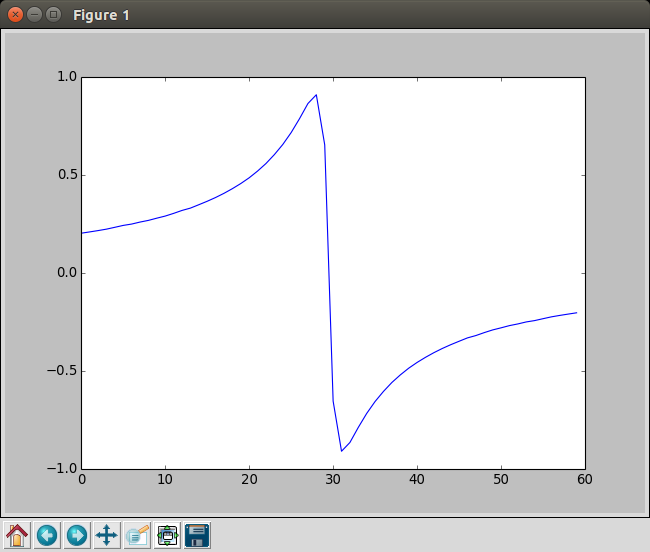
\includegraphics[width=0.75\textwidth]{1D_se.png}
\end{center}


\newpage
%\begin{lstlisting}[language=Python, caption=Plotting 2D data, frame=single,basicstyle=\small]
\subsection*{Plotting 2D data: \protect\Verb+2D\_plot\_minimal.py+}
\begin{minted}{python}
from __future__ import print_function, division
import numpy as np
import h5py
import matplotlib.pyplot as plt

f = h5py.File('adga-12345.hdf5','r')

# extract the fermionic vertex box size
iwf = f['input/iwfmax_small'][()]

dset = f['selfenergy/nonloc/dga'][()]

# plot the first band at the first fermionic frequency
# in the kz = 0 plane
f = plt.figure()

f.add_subplot(211) # 2x1 subplots
plt.pcolormesh(dset[0,0,:,:,0,iwf].imag)

f.add_subplot(212)
plt.pcolormesh(dset[0,0,:,:,0,iwf].real)

plt.show()
\end{minted}

If everything works correctly, you should get the following plot:\\
\begin{center}
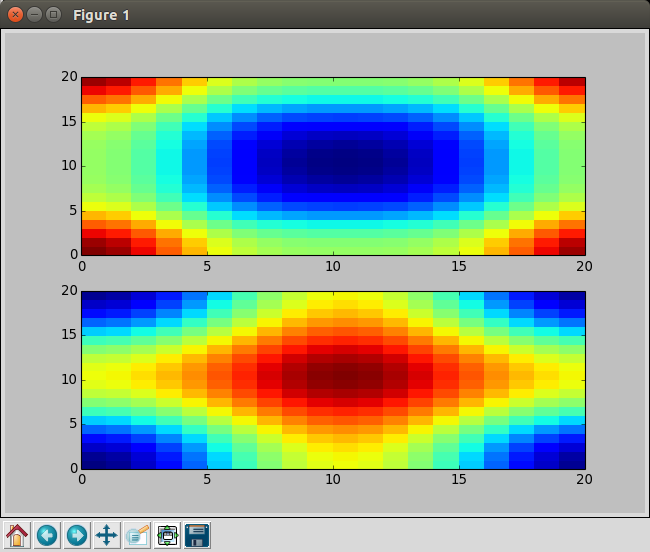
\includegraphics[width=0.75\textwidth]{se-plane.png}\\
\end{center}
If you want to make a proper plot of the full Brillouin zone, please
have a look at the script \verb=documentation/plot_scripts/2D_plot_selfenergy_plane.py=.

\newpage
\subsection*{How to build a minimal DMFT file: \protect\Verb=construct\_input\_structure.py=}
Here we assume that the user has all necessary data for starting a D$\Gamma$A run,
just not in the correct file format. The following script contains the necessary 
commands to create a minimal input file in the correct format.

\begin{minted}{python}

#! /usr/bin/env python

from __future__ import print_function, division, absolute_import
import numpy as np
import h5py

def read_1p_data(iw,siw,giw,dc,mu,beta):
    # read in your data according to your format.
    # save them in iw,siw,giw,dc,mu,beta as necessary for ADGA
    pass

def read_2p_data(group, g2):
    # read in one spin-band group of your two-particle data
    pass


read_1p_data(iw,siw,giw,dc,mu,beta)

f = h5py.File('1p-data.hdf5','w')
f['.axes/iw']=iw
f.create_group('.config')
f['.config'].attrs['general.beta']=beta
f['dmft-001/mu/value']=mu
f['dmft-001/ineq-001/dc/value']=dc
f['dmft-001/ineq-001/siw/value']=siw
f['dmft-001/ineq-001/giw/value']=giw
f.close()


g = h5py.File('2p-data.hdf5','w')

# groups holds all spin-band combinations of
# the two particle Greens function
# as strings, e.g. '00001'
for group in groups: 
    read_2p_data(group, g2)
    g['worm-001/ineq-001/g4iw-worm/'+group+'/value'] = g2
g.close()


n4iwf=g2.shape[0]//2
n4iwb=g2.shape[-1]//2

g['.axes/iwf-g4'] = np.pi/beta * (2 * np.arange(-n4iwf,n4iwf) +1)
g['.axes/iwb-g4'] = np.pi/beta * 2 * np.arange(-n4iwb,n4iwb+1)

g.close()

\end{minted}

\end{document}
